% ===============================================
% MATH 3053: Abstract Algebra I         Fall 2017
% hw_revised.tex
% Template for revised homework submission
% ===============================================
%         READ THE FOLLOWING CAREFULLY!!!
% ===============================================
% When you produce a PDF version of this document
% to turn in, change the filename to hwX-name.pdf
% replacing X with the homework assignment number
% and name with your last name.
% ===============================================


% -----------------------------------------------
% The preamble that follows can be ignored. Go on
% down to the section that says "START HERE" 
% -----------------------------------------------

\documentclass{article}

\usepackage[margin=1in]{geometry} 
\usepackage{amsmath,amsthm,amssymb}
\usepackage{tikz}
\usepackage{darkmode}
\enabledarkmode


\newcommand{\R}{\mathbb{R}}  
\newcommand{\Z}{\mathbb{Z}}
\newcommand{\N}{\mathbb{N}}
\newcommand{\Q}{\mathbb{Q}}
\newcommand{\C}{\mathbb{C}}

\newenvironment{theorem}[2][Theorem]{\begin{trivlist}
\item[\hskip \labelsep {\bfseries #1}\hskip \labelsep {\bfseries #2.}]}{\end{trivlist}}
\newenvironment{lemma}[2][Lemma]{\begin{trivlist}
\item[\hskip \labelsep {\bfseries #1}\hskip \labelsep {\bfseries #2.}]}{\end{trivlist}}
\newenvironment{exercise}[2][Exercise]{\begin{trivlist}
\item[\hskip \labelsep {\bfseries #1}\hskip \labelsep {\bfseries #2.}]}{\end{trivlist}}
\newenvironment{problem}[2][Problem]{\begin{trivlist}
\item[\hskip \labelsep {\bfseries #1}\hskip \labelsep {\bfseries #2.}]}{\end{trivlist}}
\newenvironment{question}[2][Question]{\begin{trivlist}
\item[\hskip \labelsep {\bfseries #1}\hskip \labelsep {\bfseries #2.}]}{\end{trivlist}}
\newenvironment{corollary}[2][Corollary]{\begin{trivlist}
\item[\hskip \labelsep {\bfseries #1}\hskip \labelsep {\bfseries #2.}]}{\end{trivlist}}

\newenvironment{solution}{\begin{proof}[Solution]}{\end{proof}}

\begin{document}

% ------------------------------------------ %
%                 START HERE                 %
% ------------------------------------------ %

\title{Discrete Math II} % Replace X with the appropriate number
\author{Matteo Costagliola\\Homework 2} % Replace "Author's Name" with your name

\maketitle


\begin{problem}{1} Find planar representations for each of the planar graphs in Figure 1.78.\\
    \begin{figure}[h]
        \centering
        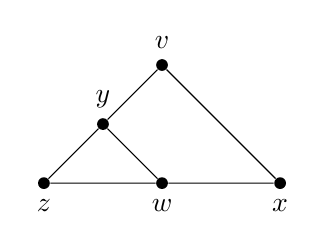
\begin{tikzpicture}[scale=3, rotate=-90]
        
            \node[fill=black, circle, inner sep=1.5pt, label=$v$] (v) at (0,-0.5) {};
            \node[fill=black, circle, inner sep=1.5pt, label=below:$x$] (x) at (0.5,0) {};
            \node[fill=black, circle, inner sep=1.5pt, label=$y$] (y) at (0.25,-0.75) {};
            \node[fill=black, circle, inner sep=1.5pt, label=below:$w$] (w) at (0.5,-0.5) {};
            \node[fill=black, circle, inner sep=1.5pt, label=below:$z$] (z) at (0.5,-1) {};

            \draw[black, thin] (v) -- (x) node[midway, above right] {};
            \draw[black, thin] (x) -- (w) node[midway, above right] {};
            \draw[black, thin] (v) -- (y) node[midway, above right] {};
            \draw[black, thin] (y) -- (z) node[midway, above right] {};
            \draw[black, thin] (w) -- (z) node[midway, above right] {};
            \draw[black, thin] (y) -- (w) node[midway, above right] {};

        \end{tikzpicture}
        %%%%%%%%%%%%%%%%%%%%%%%%%%%%%%%%%%%%
        \hspace{3cm}
        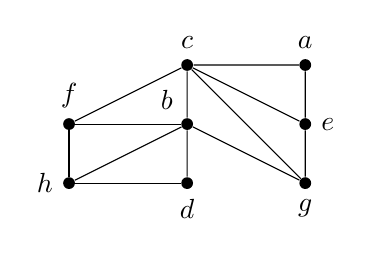
\begin{tikzpicture}[scale=3, rotate=90]
        
            \node[fill=black, circle, inner sep=1.5pt, label=left:$h$] (h) at (0,0) {};
            \node[fill=black, circle, inner sep=1.5pt, label=below:$d$] (d) at (0,-0.5) {};
            \node[fill=black, circle, inner sep=1.5pt, label=above left:$b$] (b) at (0.25,-0.5) {};
            \node[fill=black, circle, inner sep=1.5pt, label=above:$f$] (f) at (0.25,0) {};
            \node[fill=black, circle, inner sep=1.5pt, label=below:$g$] (g) at (0,-1) {};
            \node[fill=black, circle, inner sep=1.5pt, label=above:$c$] (c) at (0.5,-0.5) {};
            \node[fill=black, circle, inner sep=1.5pt, label=right:$e$] (e) at (0.25,-1) {};
            \node[fill=black, circle, inner sep=1.5pt, label=above:$a$] (a) at (0.5,-1) {};

            \draw[black, thin] (h) -- (f) node[midway, above right] {};
            \draw[black, thin] (h) -- (d) node[midway, above right] {};
            \draw[black, thin] (h) -- (b) node[midway, above right] {};
            \draw[black, thin] (d) -- (b) node[midway, above right] {};
            \draw[black, thin] (g) -- (b) node[midway, above right] {};
            \draw[black, thin] (f) -- (c) node[midway, above right] {};
            \draw[black, thin] (b) -- (c) node[midway, above right] {};
            \draw[black, thin] (g) -- (c) node[midway, above right] {};
            \draw[black, thin] (f) -- (b) node[midway, above right] {};
            \draw[black, thin] (g) -- (e) node[midway, above right] {};
            \draw[black, thin] (c) -- (e) node[midway, above right] {};
            \draw[black, thin] (a) -- (e) node[midway, above right] {};
            \draw[black, thin] (c) -- (a) node[midway, above right] {};

        \end{tikzpicture}
        \caption{Planar representations of graphs in figure 1.78}
        \end{figure}
\end{problem}
%%%%%%%%%%%%%%%%%%%%%%%%%%%
\vspace{0.25cm}
%%%%%%%%%%%%%%%%%%%%%%%%%%%
\begin{problem}{2}Draw a planar graph in which every vertex has degree exactly 5.
        \begin{figure}[h]
            \centering
            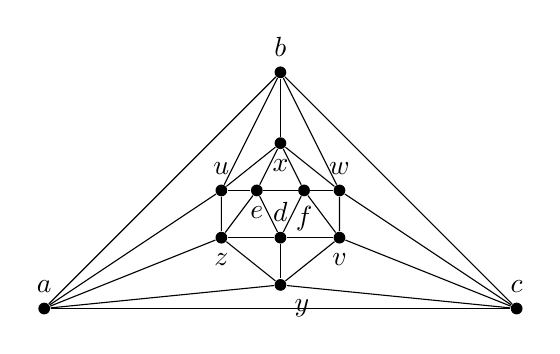
\begin{tikzpicture}[scale=3]

                \node[fill=black, circle, inner sep=1.5pt, label=$a$] (a) at (0,0) {};
                \node[fill=black, circle, inner sep=1.5pt, label=$b$] (b) at (1,1) {};
                \node[fill=black, circle, inner sep=1.5pt, label=$c$] (c) at (2,0) {};
                \node[fill=black, circle, inner sep=1.5pt, label=$d$] (d) at (1,0.3) {};
                \node[fill=black, circle, inner sep=1.5pt, label=below:$e$] (e) at (0.9,0.5) {};
                \node[fill=black, circle, inner sep=1.5pt, label=below:$f$] (f) at (1.1,0.5) {};
                \node[fill=black, circle, inner sep=1.5pt, label=below:$x$] (x) at (1,0.7) {};
                \node[fill=black, circle, inner sep=1.5pt, label=below right:$y$] (y) at (1,0.1) {};
                \node[fill=black, circle, inner sep=1.5pt, label=below:$z$] (z) at (0.75,0.3) {};
                \node[fill=black, circle, inner sep=1.5pt, label=$u$] (u) at (0.75,0.5) {};
                \node[fill=black, circle, inner sep=1.5pt, label=below:$v$] (v) at (1.25,0.3) {};
                \node[fill=black, circle, inner sep=1.5pt, label=$w$] (w) at (1.25,0.5) {};

                \draw[black, thin] (a)--(b) node[midway,above right] {};
                \draw[black, thin] (a)--(c) node[midway,above right] {};
                \draw[black, thin] (a)--(z) node[midway,above right] {};
                \draw[black, thin] (a)--(y) node[midway,above right] {};
                \draw[black, thin] (a)--(u) node[midway,above right] {};
                \draw[black, thin] (b)--(u) node[midway,above right] {};
                \draw[black, thin] (b)--(x) node[midway,above right] {};
                \draw[black, thin] (b)--(w) node[midway,above right] {};
                \draw[black, thin] (c)--(w) node[midway,above right] {};
                \draw[black, thin] (c)--(v) node[midway,above right] {};
                \draw[black, thin] (c)--(y) node[midway,above right] {};
                \draw[black, thin] (c)--(b) node[midway,above right] {};
                \draw[black, thin] (e)--(f) node[midway,above right] {};
                \draw[black, thin] (e)--(d) node[midway,above right] {};
                \draw[black, thin] (f)--(d) node[midway,above right] {};
                \draw[black, thin] (d)--(z) node[midway,above right] {};
                \draw[black, thin] (d)--(y) node[midway,above right] {};
                \draw[black, thin] (d)--(v) node[midway,above right] {};
                \draw[black, thin] (e)--(z) node[midway,above right] {};
                \draw[black, thin] (e)--(u) node[midway,above right] {};
                \draw[black, thin] (e)--(x) node[midway,above right] {};
                \draw[black, thin] (f)--(x) node[midway,above right] {};
                \draw[black, thin] (f)--(w) node[midway,above right] {};
                \draw[black, thin] (f)--(v) node[midway,above right] {};
                \draw[black, thin] (x)--(u) node[midway,above right] {};
                \draw[black, thin] (x)--(w) node[midway,above right] {};
                \draw[black, thin] (y)--(v) node[midway,above right] {};
                \draw[black, thin] (y)--(z) node[midway,above right] {};
                \draw[black, thin] (u)--(z) node[midway,above right] {};
                \draw[black, thin] (w)--(v) node[midway,above right] {};
            
            \end{tikzpicture}
        \end{figure}
\end{problem}
%%%%%%%%%%%%%%%%%%%%%%%%%%%
\vspace{0.25cm}
%%%%%%%%%%%%%%%%%%%%%%%%%%%
\begin{problem}{3} Fary and Wagner proved independently that every planar graph has a planar representation in which every edge is a straight line segment. Find such a representation for the graph in Figure 1.80.\\
    \begin{figure}[h]
        \centering
        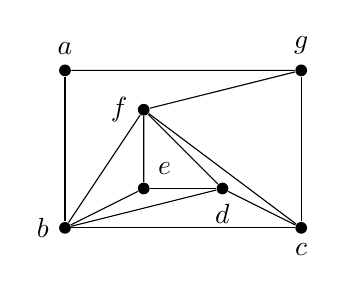
\begin{tikzpicture}[scale=5, rotate=90]
            
            \node[fill=black, circle, inner sep=1.5pt, label=$a$] (a) at (0.4,0) {};
            \node[fill=black, circle, inner sep=1.5pt, label=left:$b$] (b) at (0,0) {};
            \node[fill=black, circle, inner sep=1.5pt, label=below:$c$] (c) at (0,-0.6) {};
            \node[fill=black, circle, inner sep=1.5pt, label=below:$d$] (d) at (0.1,-0.4) {};
            \node[fill=black, circle, inner sep=1.5pt, label=above right:$e$] (e) at (0.1,-0.2) {};
            \node[fill=black, circle, inner sep=1.5pt, label=left:$f$] (f) at (0.3,-0.2) {};
            \node[fill=black, circle, inner sep=1.5pt, label=above:$g$] (g) at (0.4,-0.6) {};

            \draw[black, thin] (a) -- (b) node[midway, above right] {};
            \draw[black, thin] (b) -- (c) node[midway, above right] {};
            \draw[black, thin] (c) -- (d) node[midway, above right] {};
            \draw[black, thin] (d) -- (e) node[midway, above right] {};
            \draw[black, thin] (e) -- (f) node[midway, above right] {};
            \draw[black, thin] (f) -- (g) node[midway, above right] {};

            \draw[black, thin] (b) -- (d) node[midway, above right] {};
            \draw[black, thin] (b) -- (e) node[midway, above right] {};
            \draw[black, thin] (b) -- (f) node[midway, above right] {};
            \draw[black, thin] (a) -- (g) node[midway, above right] {};
            \draw[black, thin] (c) -- (f) node[midway, above right] {};
            \draw[black, thin] (c) -- (g) node[midway, above right] {};
            \draw[black, thin] (d) -- (f) node[midway, above right] {};

        \end{tikzpicture}
        \caption{Planar Representation with line segment edges}
    \end{figure}
    
\end{problem}
%%%%%%%%%%%%%%%%%%%%%%%%%%%
\vspace{0.25cm}
%%%%%%%%%%%%%%%%%%%%%%%%%%%
\begin{problem}{4}If planar graphs $G_{1}$ and $G_{2}$ each have $n$ vertices, $q$ edges, and $r$ regions, must the graphs be isomorphic?
    \\\textit{Counterexample}
    \begin{figure}[h]
        \centering
        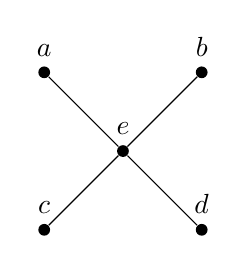
\begin{tikzpicture}[scale=2]
            
            \node[fill=black, circle, inner sep=1.5pt, label=$a$] (a) at (0,0) {};
            \node[fill=black, circle, inner sep=1.5pt, label=$b$] (b) at (1,0) {};
            \node[fill=black, circle, inner sep=1.5pt, label=$c$] (c) at (0,-1) {};
            \node[fill=black, circle, inner sep=1.5pt, label=$d$] (d) at (1,-1) {};
            \node[fill=black, circle, inner sep=1.5pt, label=$e$] (e) at (0.5,-0.5) {};

            \draw[black, thin] (e)--(a) {};
            \draw[black, thin] (e)--(b) {};
            \draw[black, thin] (e)--(c) {};
            \draw[black, thin] (e)--(d){};

        \end{tikzpicture}
        \hspace{3cm}
        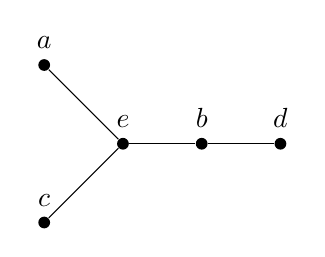
\begin{tikzpicture}[scale=2]
            
            \node[fill=black, circle, inner sep=1.5pt, label=$a$] (a) at (0,0) {};
            \node[fill=black, circle, inner sep=1.5pt, label=$b$] (b) at (1,-0.5) {};
            \node[fill=black, circle, inner sep=1.5pt, label=$c$] (c) at (0,-1) {};
            \node[fill=black, circle, inner sep=1.5pt, label=$d$] (d) at (1.5,-0.5) {};
            \node[fill=black, circle, inner sep=1.5pt, label=$e$] (e) at (0.5,-0.5) {};

            \draw[black, thin] (e)--(a) {};
            \draw[black, thin] (e)--(b) {};
            \draw[black, thin] (e)--(c) {};
            \draw[black, thin] (b)--(d) {};

        \end{tikzpicture}
        \caption{Two graphs with 5 vertices, 4 edges, and 1 region that are no isomorphic}
    \end{figure}
\end{problem}
%%%%%%%%%%%%%%%%%%%%%%%%%%%
\vspace{0.25cm}
%%%%%%%%%%%%%%%%%%%%%%%%%%%
\begin{problem}{5}Let $G$ be a connected planar graph of order less than 12. Prove that $\delta(G)\leq 4$.
    \begin{proof}
        Suppose that $\delta(G)\geq 5$. Then we have that $\sum_{v\in V}\text{deg}(v)\geq 5n$ where $n=|V|$. Since each edge is composed of a pair of vertices we also have that $2q\geq 5n$ where $q$ is the number of edges. Using the planarity condition $q\leq 3n-6$. Substituting in our found values yields $\frac{5n}{2}\leq3n-6$. Multiplying by 2 to clear denominators leaves us with $5n\leq6n-12$. Then rearranging this equation gives $n\geq12$. However we are told $G$ has $n<12$, thus we have a contradiction. Therefore a connected planar graph $G$ with order less than 12 must have $\delta(G)\leq4$.
    \end{proof}
\end{problem}
%%%%%%%%%%%%%%%%%%%%%%%%%%%
\vspace{0.25cm}
%%%%%%%%%%%%%%%%%%%%%%%%%%%
\begin{problem}{6}Let $G$ be a connected, planar, $K_{3}$-free graph of order $n\geq3$. Prove that $G$ has no more than $2n-4$ edges.
    \begin{proof}
        To say that $G$ is $K_{3}$-free means that there is no cycle of length 3. Let $\sum_{r\in R}\text{deg}(r)=2q$ be the sum of the edges bounding each region $r$. If $G$ is $K_{3}$-free then edges$(r)\geq 4$ for each region in $G$. Thus $2q\geq 4R$. Using Euler's formula $n-q+r=2$ and substituting in the found value we obtain $n-q+\frac{1}{2}q\geq2$. Clearing the denominator gives $2n-2q+q\geq4$. Solving for $q$ gives $q\leq2n-4$. Thus any connected planar graph $G$ that is $K_{3}$-free with order $n\geq3$ will have at most $2n-4$ edges.
    \end{proof}
\end{problem}
%%%%%%%%%%%%%%%%%%%%%%%%%%%
\vspace{0.25cm}
%%%%%%%%%%%%%%%%%%%%%%%%%%%
\begin{problem}{7}Prove that there is no bipartite planar graph with minimum degree at least 4.
    \begin{proof}
        If $G$ is a bipartite planar graph with $\delta(G)\geq 4$, then each region, $r$, must be bounded by at least 4 edges in order to not contain $C_{3}$. Let $D=\sum_{r\in R}\text{deg}(r)=2q$ be the sum of the number of edges bounding the regions in $G$. Since each region must be bound by at least 4 edges we have $2q\geq4R$. Solving for $R$ gives $R\geq\frac{1}{2}q$. Using Euler's formula we have $n-q+\frac{1}{2}q\geq 2$. Thus since $\delta(G)\geq4$ we have that $n\geq\delta(G)+1=5$. We then have $5-4+2=3\neq2$. Thus there is no bipartite planar graph with $\delta(G)\geq 4$.

    \end{proof}
\end{problem}










\newpage
note:\\
Suppose there exists a planar graph such that each vertex has exactly degree 5. Then $\sum_{v\in V}\text{deg}(v)=5|V|$. By the handshaking lemma --- $\sum_{v\in V}\text{deg}(v)=2|E|=5|V|$, thus $|E|=\frac{5|V|}{2}$. Using Euler's formula, $V-E+R=2$, where $E$ must be an integer, this means that $|V|$ must be even for $|E|$ to be an integer. By theorem 1.33, a planar graph with at least $|V|\geq 3$ vertices and $|E|$ edges must satisfy $|E|\leq 3|V|-6$. Substituting $|E|=\frac{5|V|}{2}$ into the inequality we see that $\frac{5|V|}{2}\leq 3|V|-6$. Multiplying by 2 yields $5|V|\leq 6|V|-12$. Then rearranging the inequality gives us $|V|\geq 12$. Revisiting Euler's formula and using the formula for the number of edges we found earlier, $|E|=\frac{5|V|}{2}$, using $|V|=12$ we see that $E=\frac{5(12)}{2}=30$. Solving for the number of regions, $R$, gives $R=2-V+E=2-12+30=20$. However a graph cannot have a negative number of regions.

% -----------------------------------------------------
% The following two environments (theorem, proof) are
% where you will enter the statement and proof of your
% first problem for this assignment.
%
% In the theorem environment, you can replace the word
% "theorem" in the \begin and \end commands with
% "exercise", "problem", "lemma", etc., depending on
% what you are submitting. Replace the "x.yz" with the
% appropriate number for your problem.
%
% If your problem does not involve a formal proof, you
% can change the word "proof" in the \begin and \end
% commands with "solution".
% -----------------------------------------------------

% -----------------------------------------------
% Ignore everything that appears below this.
% -----------------------------------------------

\end{document}
